\section{Where the ruler stops working}
\label{sec:measurement}

Every claim above rests on two graders agreeing about orderings, so we report where they stop.

\textbf{Arm-level agreement is strong.} Across all $44$ model states of the grid, the held-out
judge preserves the sign of $6{,}693$ of $8 \times \binom{44}{2} = 7{,}568$ pairwise state
$\times$ instrument contrasts ($88.4\%$); restricted to contrasts the training oracle scores at
$|\Delta| \geq 0.25$ this rises to $97.2\%$, and at $|\Delta| \geq 0.50$ to $99.3\%$. The
disagreements sit almost entirely in gaps too small to claim; every contrast in this paper is
well inside the agreeing range.

\textbf{Per-conversation agreement collapses exactly at the late $\Kf$ checkpoints.} On the
rewarded rubric Q1, per-conversation correlation between the graders has a 44-state median of
$0.855$; \GRPO-$\Kf$'s last two iterations read $\mathbf{0.487}$ and $\mathbf{0.544}$ --- the
two lowest-agreeing states in the experiment --- and \PTO-$\Kf$'s endpoint is the next cluster
down ($0.667$). \textbf{Both $\Kf$ arms lose Q1 agreement over their final two iterations;
neither $\Kz$ arm does} (Figure~\ref{fig:saturation}) --- with one training run per arm we
cannot separate ``these checkpoints'' from ``long $\Kf$ training,'' but the pattern recurring
across two different optimizers is itself evidence that it is the horizon's late-run policies,
not one optimizer's quirk.

\textbf{The mechanism is one-sided saturation of the trained-against grader.} A correlation can
collapse because conversations became uniform or because one rater ran out of range; the two are
distinguishable because only one grader's spread moves. On \GRPO-$\Kf$'s conversations, the
training oracle's per-conversation Q1 standard deviation falls monotonically from $1.336$ (base)
to $0.701$ (iteration 10; Spearman $\rho = -0.86$, $p = .001$; variance ratio $0.275$), while the
held-out judge's spread over the \emph{identical} conversations does not move ($\rho = +0.44$,
$p = .18$). Had the conversations homogenised, both spreads would have shrunk; one shrank and the
other did not, so what changed is the ruler.

\begin{figure}[t]
\centering
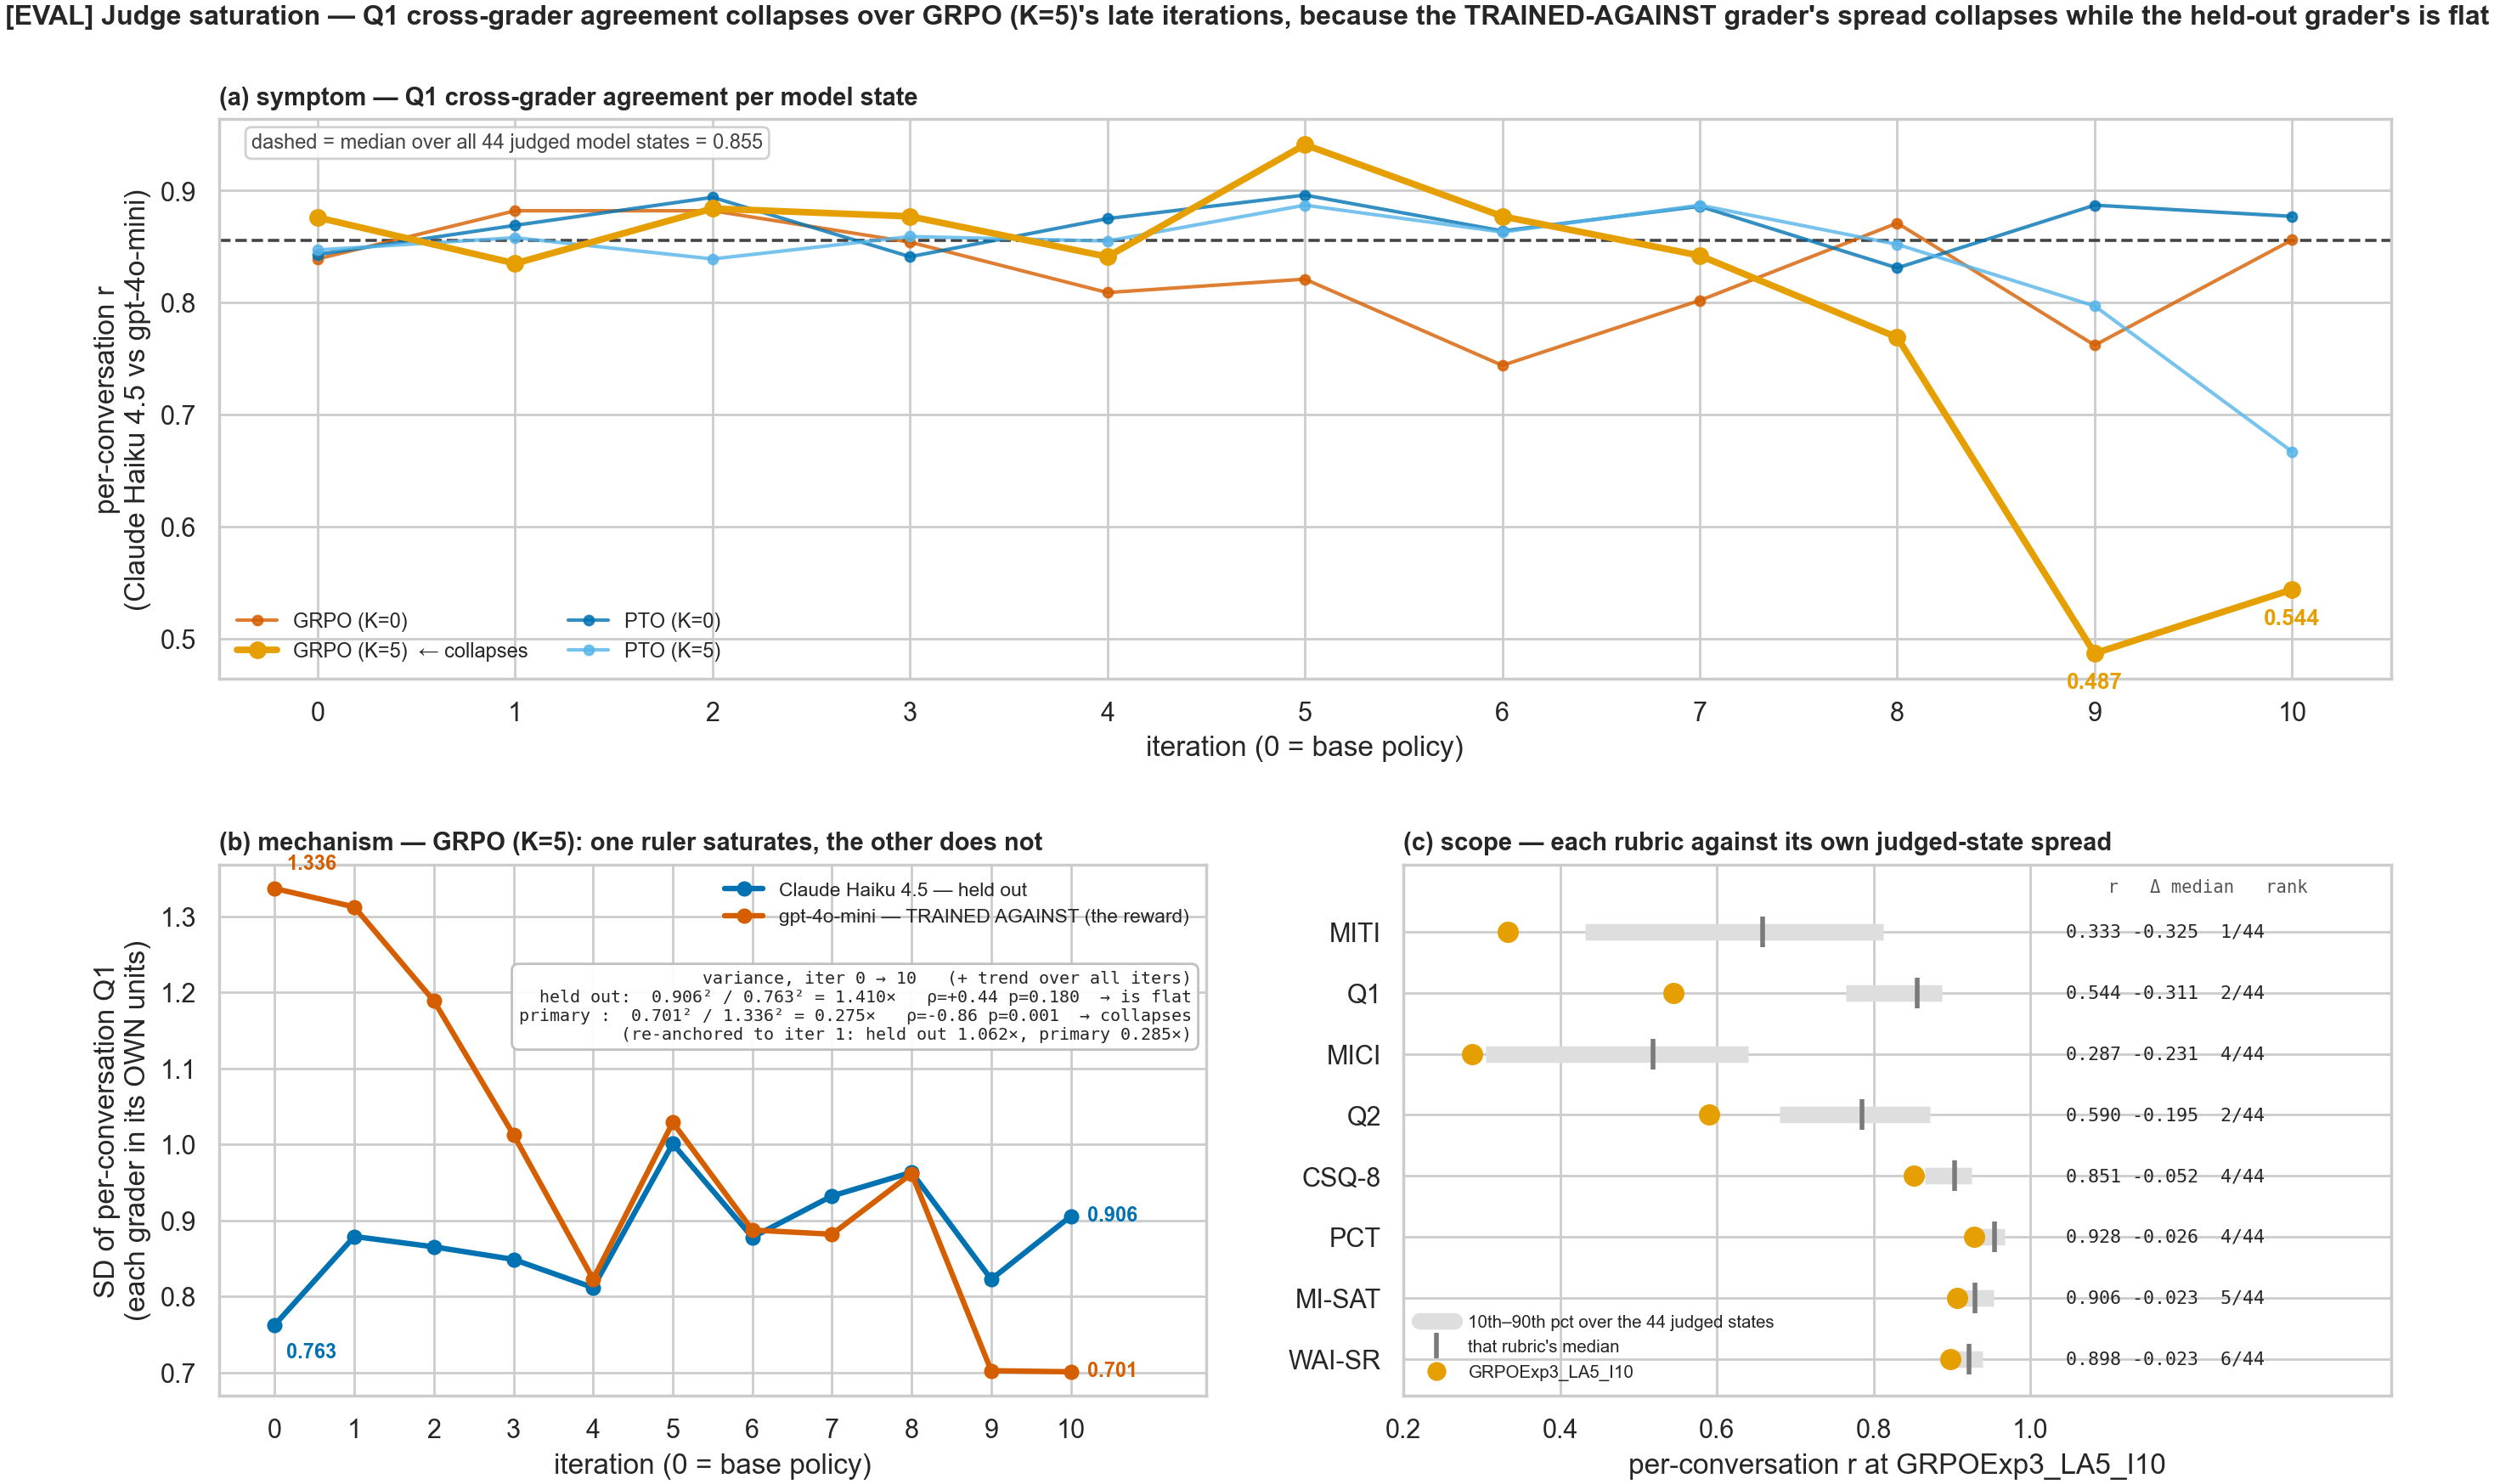
\includegraphics[width=0.98\linewidth]{figures/judge_saturation.png}
\caption{\textbf{(a)} Per-conversation cross-grader agreement on Q1 by iteration, one line per
arm, against the 44-state median: both $\Kf$ arms fall late, neither $\Kz$ arm does.
\textbf{(b)} The mechanism on the collapsing arm --- Q1 SD under each grader on the same
conversations: the training oracle's spread collapses, the held-out judge's is flat. (SD is a
spread, so the graders can share an axis; their score levels never can.) \textbf{(c)} The
collapse by rubric at the worst state, each against its own distribution.}
\label{fig:saturation}
\end{figure}

\textbf{Consequences for the claims above.} Arm-level contrasts survive --- the held-out judge,
the one still discriminating, is the grader under which the interaction is \emph{largest} --- but
three kinds of claims are marked wherever they appear: per-conversation claims about late $\Kf$
checkpoints on the rewarded and behaviour-coding rubrics; absolute endpoint levels near the top
of the training oracle's compressed range (\GRPO-$\Kf$'s $4.52$ on a 1--5 scale should be read as
``near this grader's ceiling''); and the training-oracle side of the two-winners comparison in
\S\ref{ssec:winners}, which is precisely a contrast between a state this grader has saturated on
and one it has not. This failure mode --- one judge supplying both the reward and the reported
outcome, then quietly losing its discriminative range on exactly the checkpoints being reported
--- is invisible to arm-level agreement statistics, and we suspect it is common; the cheap
diagnostic is to track the training grader's per-conversation \emph{variance} by iteration, not
just its mean.
